
% AUTHOR_body.tex
% Prepared by C. Pinon (cjpinon@implicature.xyz) for EISS 13 (see
% https://implicature.xyz/eiss13/)
% 2020-02-02

% Please use this file (which you should rename) for the main ("body")
% part of your paper. Be sure to compile the master file, not this one.

% Put your main text here. Recall that the references are in a separate
% file. And recall also that "\begin{document}" and "\end{document}"
% have already been inserted, which means that you can begin immediately
% with the first section.

\section{Introduction}\label{sec:1}

In this paper, we will show how semantics and pragmatics reduce to
syntax (or the other way around, see \citealt{Kamp:1973,Searle:1964}) \ldots 

\section{Typsetting stuff}

Here, we show how frequently needed linguistic elements can be typeset in \LaTeX. These instructions should cover most of your needs. 

\subsection{Linguistic examples with glosses and translations}

For examples, use \textbf{linguex}, and for glossing morphological categories, please refer to the Leipzig Glossing Rules.

\ex. Swiss German \citep[][346]{hodler69}
\gll win er der Namen Gottes het usgsprochn-a ghabe\\
when he the name.\textsc{m.sg} God.\textsc{gen} has pronounced-\textsc{m.sg} had\\
`once he had pronounced the name of God'

\Next shows how you can typeset examples with several subexamples. Please avoid, if at all possible, examples that are cut from their translation. You may want to force a new page, if this cannot be avoided. In order to refer back or forth to an example, you can either do it like \ref{ex:1} and \ref{ex:2}, or rather with the shorthands \Next[c] or \Last. Either will work, but only the first version will require that you add a \emph{label} to the example, as we have done below.


\ex. \label{ex:1}\a. \label{ex:2}First example
\b. Second
\bg. Dies ist ein schönes Beispiel mit einer Glose.\\
This is a beautiful example with a gloss.\\
\a. `Some translation'
\b. `Some other'
\z.
\b. Fourth

You can refer back to examples like \ref{ex:1} and \ref{ex:2}.

\subsection{Trees}

In order to make trees, use the \textbf{forest} package.

% LaTeX doesn't care how you arrange the tree in the source code, but for your won sake, you want probably want to write something as follows:
\ex. \begin{forest}
[S 
  [DP [D [ Ce\\\footnotesize{This} ] ]
      [NP [AP [A [ petit\\\footnotesize{small} ] ] ]
          [N [ arbre\\\footnotesize{tree} ] ] ] ]
  [VP [V [ est\\\footnotesize{is} ] ]
      [AP [AdvP [Adv [ très\\\footnotesize{very} ] ] ]
          [A [ joli\\\footnotesize{nice} ] ] ] ] ]
\end{forest}

You can also make a more involved example, with arrows, as is illustrated in \NNext. Ideally, you would want to avoid big spaces (you can adjust the size of the tree, if this is necessary, as we have done in \Next for \Last). 

\ex. \small{
\begin{forest}
[S 
  [DP [D [ Ce\\\footnotesize{This} ] ]
      [NP [AP [A [ petit\\\footnotesize{small} ] ] ]
          [N [ arbre\\\footnotesize{tree} ] ] ] ]
  [VP [V [ est\\\footnotesize{is} ] ]
      [AP [AdvP [Adv [ très\\\footnotesize{very} ] ] ]
          [A [ joli\\\footnotesize{nice} ] ] ] ] ]
\end{forest}
}


\ex.  \label{ex:rp-structure} 
\footnotesize{%
\begin{forest} for tree={l=10mm, l sep=0}
   [AuxP, name=top 
      [beP [RP 
              [DP [John] ] 
              [R$'$ [withP  
                       [RP [DP [hair] ] 
                           [R$'$ [AP [VP ] 
                                     [A [ colored, name=cellar ] ] ] 
                                 [R] ] ] 
                        [with, name=source] ] 
                    [R, name=c1] ] ] 
            [be, name=c2]   ]  
      [Aux [ has ] ] ]
    % and now, we draw some arrows  
   \draw[->,color=red,very thick,dotted] (source) to[out=east,in=south east] (c1);
   \draw[->,color=blue,ultra thick,dashed] (c1) to[out=east,in=south east] (c2);
   \draw [-{Latex[length=2.5mm]},color=purple,ultra thick,%
          postaction={decorate,decoration={text along path,%
          text align=center,raise=-2.5ex, text color = purple,%
          text={{Because why the hell not}}}}] (cellar) to[out=east,in=east] (top);
\end{forest}}


\subsection{AVMs}

For avms, we use \textbf{langsci-avm}.

\ex. \avm{[ attr1 & \1\\
attr2 & \2[attr3 & val3\\
attr4 & val4] ]}

You can combine \textbf{forest} and \textbf{langsci-avm}:

\ex. \begin{forest}
[A [B] [{\avm{[attr1 & val1\\
attr2 & val2\\
attr3 & val3]}} ] ]
\end{forest}l

\subsection{Tables}

For tables, we use the \textbf{booktabs}-environment, as illustrated in Table \ref{tab:article-systems}. 



%\textbf{Question: do we insist that tables are put in a table-environment?}

\begin{table}
 \centering
 \begin{tabular}[t]{lr}
  \toprule
  Type of language                     & Number \\
  \midrule
  No articles at all                   & 198    \\
  Both indefinite and definite article & 154    \\
  Definite, but no indefinite article  & 89     \\
  Indefinite, but no definite article  & 40     \\
  \midrule
  Total                                & 481    \\
  \bottomrule                                       
\end{tabular}
  \caption{Article Systems in the World's Languages according to \emph{WALS}}
  \label{tab:article-systems}
\end{table}

\subsection{Figures}

And finally, you can also add figures. Figures are floats in \LaTeX{}, so they might end up on another page. When adding a figure, please make sure that the picture is in a high enough resolution (we recommend 300dpi or more), and that you have the right to include the picture.

\begin{figure}
    \centering
    % you might need to adjust the width of the picture
    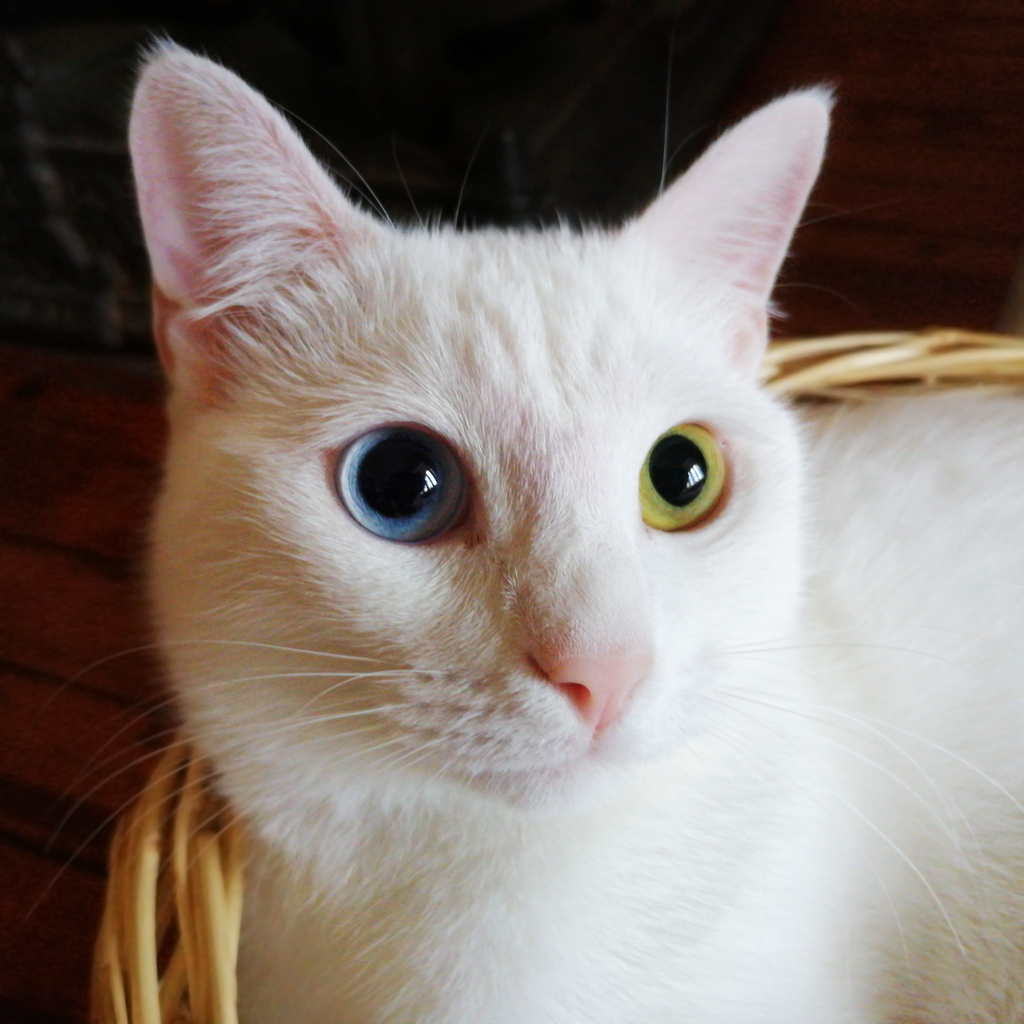
\includegraphics[width=0.4\textwidth]{cat.png}
    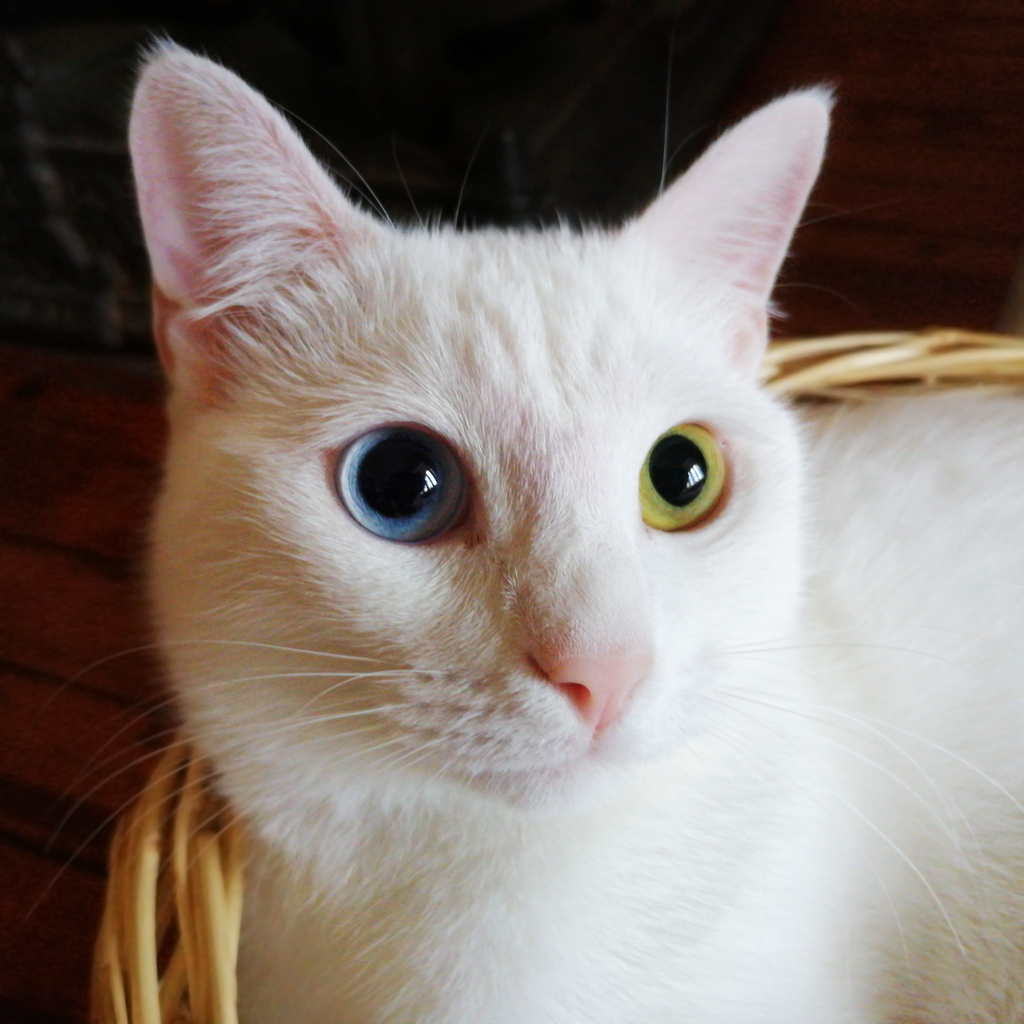
\includegraphics[width=0.4\textwidth]{cat.png}
    \caption{A cute cat and its identical twin (not sure if this is relevant)}
    \label{fig:my_cat}
\end{figure}

As usual, you can refer back to Figure \ref{fig:my_cat}.\footnote{Source of the cat: \href{https://commons.wikimedia.org/wiki/File:VAN_CAT.png}{https://commons.wikimedia.org/wiki/File:VAN\_CAT.png}.}

\subsection{References}

For references, we use \textbf{biblatex}. You can use the format familiar familiar from natbib. For instance, it is no problem to say that \citet[451]{Szadrowsky:1936} claims something, but I am not sure whether \citet[70]{Kamp:1973} would agree (or \citealt[50]{Searle:1964}, by that matter).


\section{Limitations}

As of now, we only support 5 authors. If your paper has more than 5 authors, please get in touch with us.

You can no longer compile to dvi. This is not something we intend to change.


%%%%%%%%%%
%% The official end of this file
%%%%%%%%%%

%%% Local Variables:
%%% mode: latex
%%% TeX-master: "main"
%%% End:
